
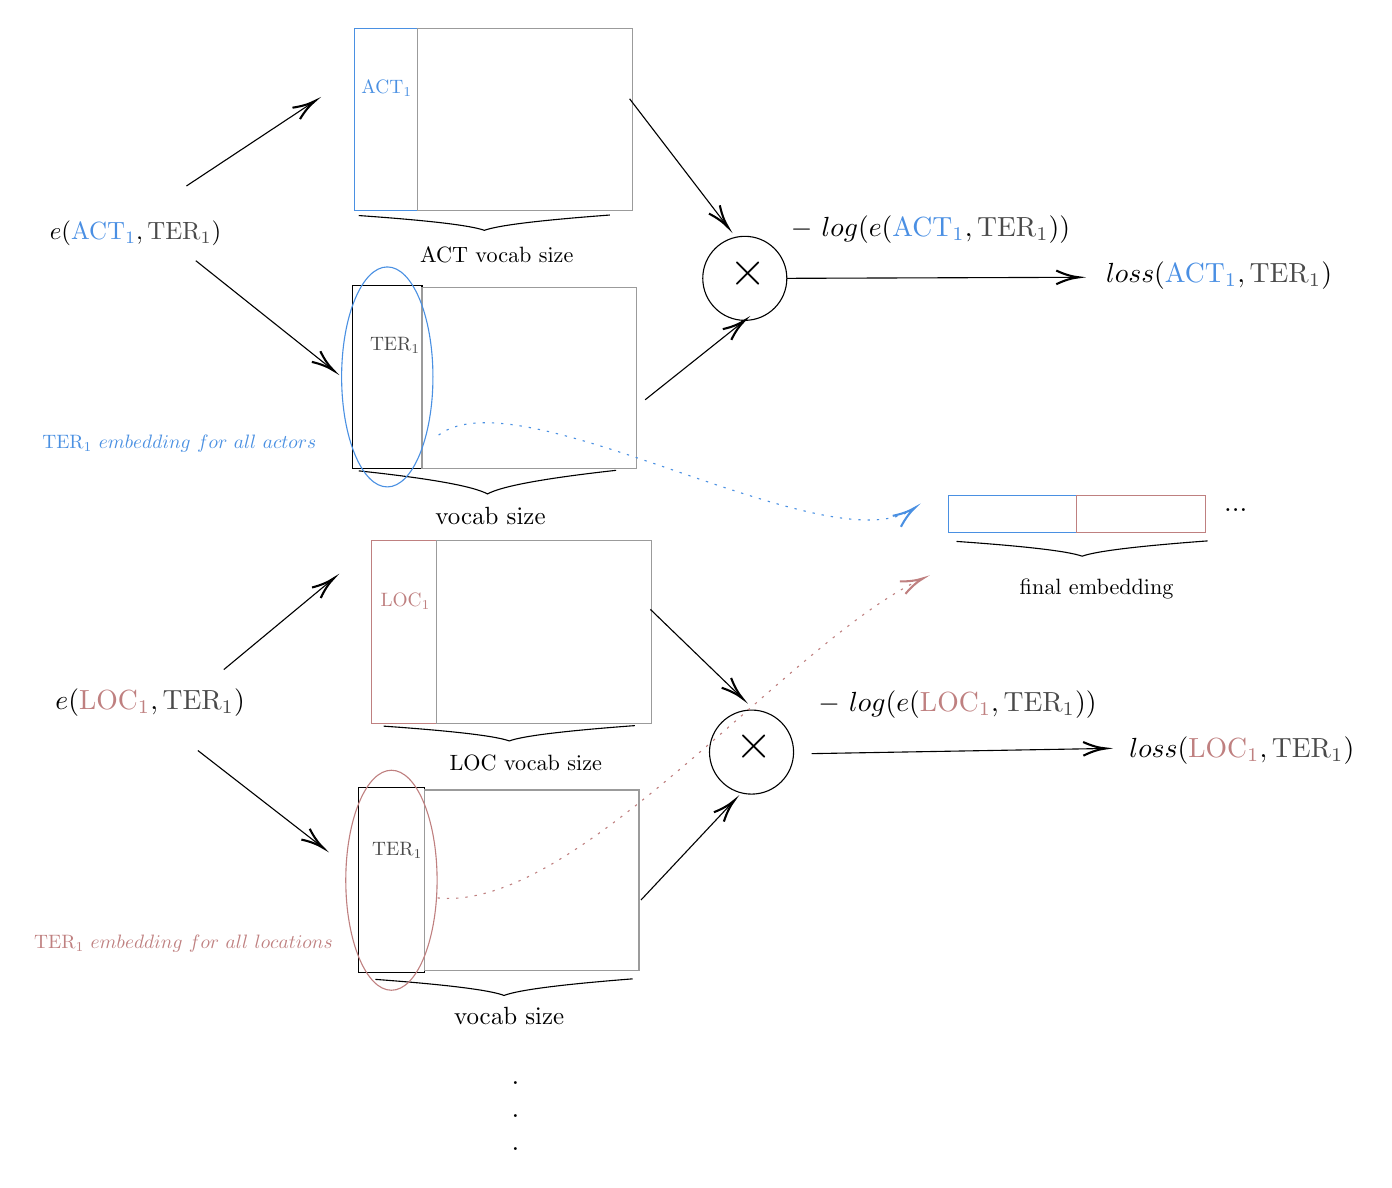
\begin{tikzpicture}[x=0.75pt,y=0.75pt,yscale=-1,xscale=1]
%uncomment if require: \path (0,573); %set diagram left start at 0, and has height of 573

%Straight Lines [id:da8462658923678936] 
\draw    (373.75,127.5) -- (512.5,127.01) ;
\draw [shift={(514.5,127)}, rotate = 539.8] [color={rgb, 255:red, 0; green, 0; blue, 0 }  ][line width=0.75]    (10.93,-3.29) .. controls (6.95,-1.4) and (3.31,-0.3) .. (0,0) .. controls (3.31,0.3) and (6.95,1.4) .. (10.93,3.29)   ;

%Straight Lines [id:da7617487325981105] 
\draw    (84.5,83) -- (144.83,43.1) ;
\draw [shift={(146.5,42)}, rotate = 506.52] [color={rgb, 255:red, 0; green, 0; blue, 0 }  ][line width=0.75]    (10.93,-3.29) .. controls (6.95,-1.4) and (3.31,-0.3) .. (0,0) .. controls (3.31,0.3) and (6.95,1.4) .. (10.93,3.29)   ;

%Shape: Rectangle [id:dp8786220898343642] 
\draw  [color={rgb, 255:red, 74; green, 144; blue, 226 }  ,draw opacity=1 ] (165.5,7) -- (196,7) -- (196,95) -- (165.5,95) -- cycle ;
%Shape: Rectangle [id:dp050244261524351685] 
\draw   (164.5,131) -- (198,131) -- (198,219) -- (164.5,219) -- cycle ;
%Shape: Rectangle [id:dp3746715403761587] 
\draw  [color={rgb, 255:red, 155; green, 155; blue, 155 }  ,draw opacity=1 ] (196,7) -- (299.5,7) -- (299.5,95) -- (196,95) -- cycle ;
%Shape: Rectangle [id:dp7065974278500844] 
\draw  [color={rgb, 255:red, 155; green, 155; blue, 155 }  ,draw opacity=1 ] (198,132) -- (301.5,132) -- (301.5,219) -- (198,219) -- cycle ;
\draw   (291.5,220) .. controls (257.06,223.82) and (236.4,227.61) .. (229.52,231.37) .. controls (222.63,227.64) and (201.95,223.93) .. (167.5,220.26) ;
\draw   (288.5,97) .. controls (254.9,99.49) and (234.73,101.94) .. (228.02,104.37) .. controls (221.29,101.97) and (201.12,99.6) .. (167.5,97.25) ;
%Shape: Ellipse [id:dp6737086825146243] 
\draw   (333.25,127.5) .. controls (333.25,116.32) and (342.32,107.25) .. (353.5,107.25) .. controls (364.68,107.25) and (373.75,116.32) .. (373.75,127.5) .. controls (373.75,138.68) and (364.68,147.75) .. (353.5,147.75) .. controls (342.32,147.75) and (333.25,138.68) .. (333.25,127.5) -- cycle ;
%Straight Lines [id:da8660824939172656] 
\draw    (305.5,186) -- (351.94,149) ;
\draw [shift={(353.5,147.75)}, rotate = 501.45] [color={rgb, 255:red, 0; green, 0; blue, 0 }  ][line width=0.75]    (10.93,-3.29) .. controls (6.95,-1.4) and (3.31,-0.3) .. (0,0) .. controls (3.31,0.3) and (6.95,1.4) .. (10.93,3.29)   ;

%Straight Lines [id:da7508477813347889] 
\draw    (298,41) -- (344.28,101.41) ;
\draw [shift={(345.5,103)}, rotate = 232.54] [color={rgb, 255:red, 0; green, 0; blue, 0 }  ][line width=0.75]    (10.93,-3.29) .. controls (6.95,-1.4) and (3.31,-0.3) .. (0,0) .. controls (3.31,0.3) and (6.95,1.4) .. (10.93,3.29)   ;

%Straight Lines [id:da41186766888830917] 
\draw    (90,355) -- (148.92,400.77) ;
\draw [shift={(150.5,402)}, rotate = 217.84] [color={rgb, 255:red, 0; green, 0; blue, 0 }  ][line width=0.75]    (10.93,-3.29) .. controls (6.95,-1.4) and (3.31,-0.3) .. (0,0) .. controls (3.31,0.3) and (6.95,1.4) .. (10.93,3.29)   ;

%Straight Lines [id:da756757421049947] 
\draw    (102.5,316) -- (153.96,273.28) ;
\draw [shift={(155.5,272)}, rotate = 500.3] [color={rgb, 255:red, 0; green, 0; blue, 0 }  ][line width=0.75]    (10.93,-3.29) .. controls (6.95,-1.4) and (3.31,-0.3) .. (0,0) .. controls (3.31,0.3) and (6.95,1.4) .. (10.93,3.29)   ;

%Shape: Rectangle [id:dp7496096523719977] 
\draw  [color={rgb, 255:red, 191; green, 128; blue, 128 }  ,draw opacity=1 ] (173.5,254) -- (205,254) -- (205,342) -- (173.5,342) -- cycle ;
%Shape: Rectangle [id:dp29079820780295873] 
\draw   (167.5,373) -- (199,373) -- (199,462) -- (167.5,462) -- cycle ;
%Shape: Rectangle [id:dp7037244075177795] 
\draw  [color={rgb, 255:red, 155; green, 155; blue, 155 }  ,draw opacity=1 ] (205,254) -- (308.5,254) -- (308.5,342) -- (205,342) -- cycle ;
%Shape: Rectangle [id:dp9036303150371852] 
\draw  [color={rgb, 255:red, 155; green, 155; blue, 155 }  ,draw opacity=1 ] (199,374) -- (302.5,374) -- (302.5,461) -- (199,461) -- cycle ;
\draw   (299.5,465) .. controls (265.06,467.7) and (244.4,470.36) .. (237.52,473) .. controls (230.62,470.39) and (209.95,467.81) .. (175.5,465.26) ;
%Shape: Ellipse [id:dp8163310771028671] 
\draw   (336.5,355.75) .. controls (336.5,344.57) and (345.57,335.5) .. (356.75,335.5) .. controls (367.93,335.5) and (377,344.57) .. (377,355.75) .. controls (377,366.93) and (367.93,376) .. (356.75,376) .. controls (345.57,376) and (336.5,366.93) .. (336.5,355.75) -- cycle ;
%Straight Lines [id:da7151838332560307] 
\draw    (303.5,427) -- (347.13,380.46) ;
\draw [shift={(348.5,379)}, rotate = 493.15] [color={rgb, 255:red, 0; green, 0; blue, 0 }  ][line width=0.75]    (10.93,-3.29) .. controls (6.95,-1.4) and (3.31,-0.3) .. (0,0) .. controls (3.31,0.3) and (6.95,1.4) .. (10.93,3.29)   ;

%Straight Lines [id:da7567579902621562] 
\draw    (308,287) -- (351.06,328.61) ;
\draw [shift={(352.5,330)}, rotate = 224.02] [color={rgb, 255:red, 0; green, 0; blue, 0 }  ][line width=0.75]    (10.93,-3.29) .. controls (6.95,-1.4) and (3.31,-0.3) .. (0,0) .. controls (3.31,0.3) and (6.95,1.4) .. (10.93,3.29)   ;

\draw   (300.5,343) .. controls (266.9,345.49) and (246.73,347.94) .. (240.02,350.37) .. controls (233.29,347.97) and (213.12,345.6) .. (179.5,343.25) ;
%Shape: Ellipse [id:dp644954323435236] 
\draw  [color={rgb, 255:red, 74; green, 144; blue, 226 }  ,draw opacity=1 ] (159.25,175) .. controls (159.25,145.73) and (169.1,122) .. (181.25,122) .. controls (193.4,122) and (203.25,145.73) .. (203.25,175) .. controls (203.25,204.27) and (193.4,228) .. (181.25,228) .. controls (169.1,228) and (159.25,204.27) .. (159.25,175) -- cycle ;
%Shape: Ellipse [id:dp6409900194653708] 
\draw  [color={rgb, 255:red, 191; green, 128; blue, 128 }  ,draw opacity=1 ] (161.25,417.5) .. controls (161.25,388.23) and (171.1,364.5) .. (183.25,364.5) .. controls (195.4,364.5) and (205.25,388.23) .. (205.25,417.5) .. controls (205.25,446.77) and (195.4,470.5) .. (183.25,470.5) .. controls (171.1,470.5) and (161.25,446.77) .. (161.25,417.5) -- cycle ;
%Curve Lines [id:da9512597890650365] 
\draw [color={rgb, 255:red, 74; green, 144; blue, 226 }  ,draw opacity=1 ] [dash pattern={on 0.84pt off 2.51pt}]  (206,203) .. controls (245.6,173.3) and (392.52,266.11) .. (434.27,238.86) ;
\draw [shift={(435.5,238)}, rotate = 503.13] [color={rgb, 255:red, 74; green, 144; blue, 226 }  ,draw opacity=1 ][line width=0.75]    (10.93,-3.29) .. controls (6.95,-1.4) and (3.31,-0.3) .. (0,0) .. controls (3.31,0.3) and (6.95,1.4) .. (10.93,3.29)   ;

%Curve Lines [id:da9524151170146553] 
\draw [color={rgb, 255:red, 191; green, 128; blue, 128 }  ,draw opacity=1 ] [dash pattern={on 0.84pt off 2.51pt}]  (205.5,426) .. controls (273.16,432.97) and (374.48,302.32) .. (438.54,272.44) ;
\draw [shift={(439.5,272)}, rotate = 515.62] [color={rgb, 255:red, 191; green, 128; blue, 128 }  ,draw opacity=1 ][line width=0.75]    (10.93,-3.29) .. controls (6.95,-1.4) and (3.31,-0.3) .. (0,0) .. controls (3.31,0.3) and (6.95,1.4) .. (10.93,3.29)   ;

%Shape: Rectangle [id:dp16117395603804296] 
\draw  [color={rgb, 255:red, 74; green, 144; blue, 226 }  ,draw opacity=1 ] (451.5,232) -- (513.5,232) -- (513.5,250) -- (451.5,250) -- cycle ;
%Shape: Rectangle [id:dp3203328454470151] 
\draw  [color={rgb, 255:red, 191; green, 128; blue, 128 }  ,draw opacity=1 ] (513.5,232) -- (575.5,232) -- (575.5,250) -- (513.5,250) -- cycle ;
%Straight Lines [id:da7598518294258658] 
\draw    (89,119) -- (153.94,170.75) ;
\draw [shift={(155.5,172)}, rotate = 218.55] [color={rgb, 255:red, 0; green, 0; blue, 0 }  ][line width=0.75]    (10.93,-3.29) .. controls (6.95,-1.4) and (3.31,-0.3) .. (0,0) .. controls (3.31,0.3) and (6.95,1.4) .. (10.93,3.29)   ;

%Straight Lines [id:da44947577411300443] 
\draw    (385.75,356.5) -- (525.5,354.04) ;
\draw [shift={(527.5,354)}, rotate = 538.99] [color={rgb, 255:red, 0; green, 0; blue, 0 }  ][line width=0.75]    (10.93,-3.29) .. controls (6.95,-1.4) and (3.31,-0.3) .. (0,0) .. controls (3.31,0.3) and (6.95,1.4) .. (10.93,3.29)   ;

\draw   (576.5,254) .. controls (542.9,256.49) and (522.73,258.94) .. (516.02,261.37) .. controls (509.29,258.97) and (489.12,256.6) .. (455.5,254.25) ;

% Text Node
\draw (60,106) node [scale=0.9] [align=left] {$e (\textcolor[rgb]{0.29,0.56,0.89}{\mathrm{ACT}}\textcolor[rgb]{0.29,0.56,0.89}{_{1}} ,\textcolor[rgb]{0.29,0.29,0.29}{\mathrm{TER}_{1}})$};
% Text Node
\draw (181,36) node [scale=0.7,color={rgb, 255:red, 74; green, 144; blue, 226 }  ,opacity=1 ]  {$\mathrm{ACT}_{1}$};
% Text Node
\draw (582,126) node  [align=left] {$loss(\textcolor[rgb]{0.29,0.56,0.89}{\mathrm{ACT}}\textcolor[rgb]{0.29,0.56,0.89}{_{1}} ,\textcolor[rgb]{0.29,0.29,0.29}{\mathrm{TER}_{1}})$};
% Text Node
\draw (185,160) node [scale=0.7,color={rgb, 255:red, 74; green, 74; blue, 74 }  ,opacity=1 ]  {$\mathrm{TER}_{1}$};
% Text Node
\draw (234,116) node [scale=0.8] [align=left] {ACT vocab size};
% Text Node
\draw (231,242) node [scale=0.9] [align=left] {vocab size};
% Text Node
\draw (67,332) node  [align=left] {$e (\textcolor[rgb]{0.75,0.5,0.5}{\mathrm{LOC}_{1}} ,\textcolor[rgb]{0.29,0.29,0.29}{\mathrm{TER}_{1}})$};
% Text Node
\draw (190,283) node [scale=0.7,color={rgb, 255:red, 191; green, 128; blue, 128 }  ,opacity=1 ]  {$\mathrm{LOC}_{1}$};
% Text Node
\draw (186,403) node [scale=0.7,color={rgb, 255:red, 74; green, 74; blue, 74 }  ,opacity=1 ]  {$\mathrm{TER}_{1}$};
% Text Node
\draw (248,361) node [scale=0.8] [align=left] {LOC vocab size};
% Text Node
\draw (240,483) node [scale=0.9] [align=left] {vocab size};
% Text Node
\draw (243,531) node  [align=left] {.\\.\\.};
% Text Node
\draw (81,207) node [scale=0.7,color={rgb, 255:red, 74; green, 144; blue, 226 }  ,opacity=1 ]  {$\mathrm{TER}_{1} \ embedding\ for\ all\ actors$};
% Text Node
\draw (83,448) node [scale=0.7,color={rgb, 255:red, 191; green, 128; blue, 128 }  ,opacity=1 ]  {$\mathrm{TER}_{1} \ embedding\ for\ all\ locations$};
% Text Node
\draw (590,239) node  [align=left] {...};
% Text Node
\draw (443,104) node  [align=left] {$-\ log( e (\textcolor[rgb]{0.29,0.56,0.89}{\mathrm{ACT}}\textcolor[rgb]{0.29,0.56,0.89}{_{1}} ,\textcolor[rgb]{0.29,0.29,0.29}{\mathrm{TER}_{1}}))$};
% Text Node
\draw (593,355) node  [align=left] {$loss(\textcolor[rgb]{0.75,0.5,0.5}{\mathrm{LOC}_{1}} ,\textcolor[rgb]{0.29,0.29,0.29}{\mathrm{TER}_{1}})$};
% Text Node
\draw (456,333) node  [align=left] {$-\ log( e (\textcolor[rgb]{0.75,0.5,0.5}{\mathrm{LOC}_{1}} ,\textcolor[rgb]{0.29,0.29,0.29}{\mathrm{TER}_{1}}))$};
% Text Node
\draw (523,277) node [scale=0.8] [align=left] {final embedding};
% Text Node
\draw (355,125) node [scale=1.7280000000000002]  {$\times $};
% Text Node
\draw (358,353) node [scale=1.7280000000000002]  {$\times $};


\end{tikzpicture}


